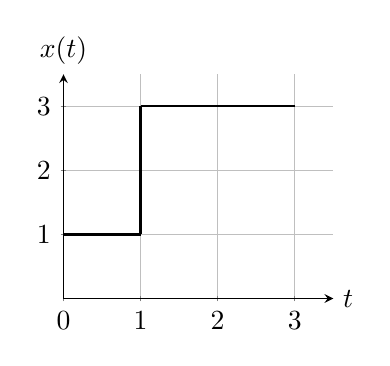
\begin{tikzpicture}
	\begin{axis}[
		xscale = 0.5,
		yscale = 0.5,
		xmin= 0, xmax = 3.5,
		ymin= 0, ymax = 3.5,
		axis x line=bottom,
		axis y line=center,
		xtick = {0,1,2, 3},
		ytick = {1, 2, 3},
		xlabel=$t$, xlabel style={at={(ticklabel* cs:1)}, anchor= west},
		ylabel=$x(t)$, ylabel style={at={(ticklabel* cs:1)}, anchor=south},
		grid=both,
		]
		\addplot[domain=0:1, thick] (\x, 1);
		\addplot[domain=1:3, thick] (\x, 3);
		\draw[thick] (axis cs:1,1) -- (axis cs:1,3);
        \end{axis}
\end{tikzpicture} 